\chapter{Workflow and Customer Journey for Coffee Chain ERP System}

\section*{Introduction}
This chapter describes the workflow and customer journey in the Coffee Chain ERP system. The system is designed to manage coffee outlets, menu items, sales orders, and customer information. The goal is to provide a clear understanding of how users (staff and administrators) interact with the system and how sale customers experience the ordering process.

\section*{System Entities}
The main entities in the Coffee Chain ERP system are:

\begin{itemize}
    \item \textbf{Coffee Outlet (\texttt{coffee.outlet})}: Represents a coffee outlet in the chain.
    \item \textbf{Outlet Owner (\texttt{res.partner})}: Represents the owner of a coffee outlet.
    \item \textbf{Coffee Menu Item (\texttt{coffee.menu.item})}: Represents drinks and snacks available for order.
    \item \textbf{Sale Customer (\texttt{res.partner})}: Represents the end customer purchasing products at the outlet.
    \item \textbf{Sale Order (\texttt{sale.order})}: Represents a customer's order in the system.
    \item \textbf{CRM Lead (\texttt{crm.lead})}: Optional linkage for sales leads and customer management.
\end{itemize}

\section*{Workflow Sequence}
The workflow represents the operations performed by administrators and staff for managing outlets, menu items, customers, and sales orders.

\subsection*{Administrator Workflow}
Administrators are responsible for setting up outlets, outlet owners, and menu items. The workflow is as follows:

\begin{enumerate}
    \item Create or manage \textbf{Outlet Owner} (\texttt{res.partner}).
    \item Create or view a \textbf{Coffee Outlet} and assign it to an outlet owner.
    \item Create \textbf{Menu Items} (drinks and snacks) that can later be added to customer orders.
    \item Create or manage \textbf{Sale Customers} (\texttt{res.partner}) who purchase items at the outlet.
    \item Optionally link \textbf{CRM Leads} to track customer interactions.
\end{enumerate}

\begin{figure}[H]
    \centering
    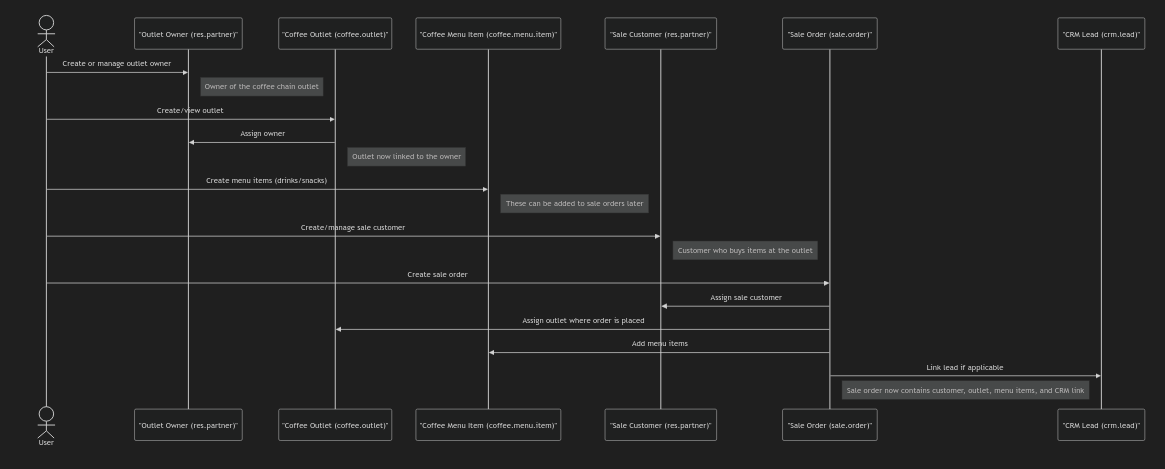
\includegraphics[width=0.85\textwidth]{diagrams/sequence.png}
    \caption{Administrator Workflow Sequence Diagram}
\end{figure}

\section*{Customer Journey}
The customer journey demonstrates how a sale customer interacts with the coffee outlet via the staff (barista) using the POS system.

\subsection*{Steps in the Customer Journey}
\begin{enumerate}
    \item Customer approaches the outlet and places an order with the staff.
    \item Staff identifies the outlet where the order is being placed.
    \item Staff adds the selected menu items to a \textbf{Sale Order}.
    \item Sale order is linked to the outlet and optionally to a CRM lead.
    \item Customer makes payment to the staff.
    \item Staff confirms the order and issues a receipt.
    \item Sale is recorded in the system, including customer details, menu items, outlet, and CRM link if applicable.
\end{enumerate}

\begin{figure}[H]
    \centering
    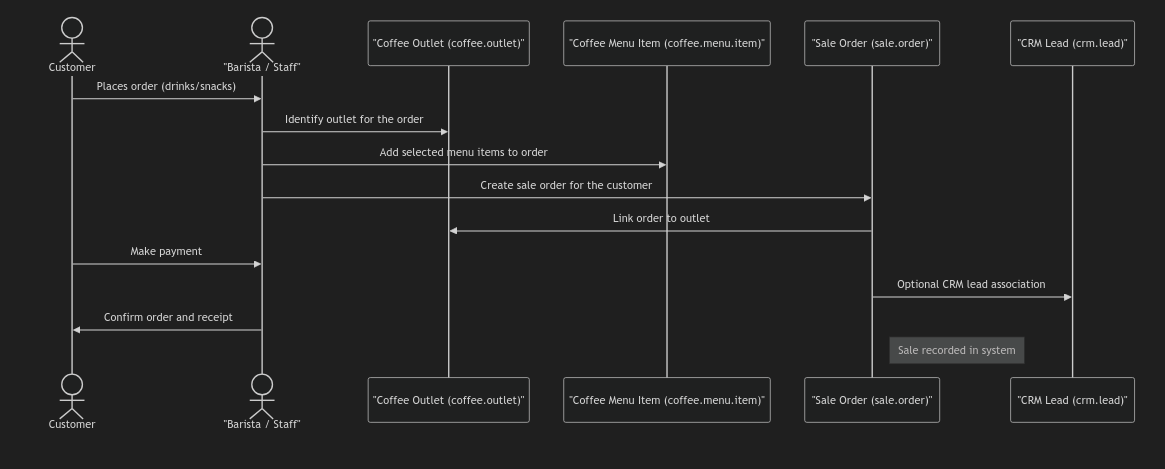
\includegraphics[width=0.85\textwidth]{diagrams/customer_journey.png}
    \caption{Customer Journey Sequence Diagram}
\end{figure}


This chapter provided a detailed workflow and customer journey for the Coffee Chain ERP system. By separating the \textbf{administrator workflow} from the \textbf{customer journey}, the system clearly defines responsibilities and interactions:

\begin{itemize}
    \item Administrators manage outlets, owners, and menu items.
    \item Staff (baristas) enter orders and process payments on behalf of customers.
    \item Sale orders record all interactions with outlets, menu items, customers, and optionally CRM leads.
\end{itemize}

